\documentclass[preprint]{aastex}

\usepackage{float}
\bibliographystyle{apj}

\begin{document}

\title{The dimensionality of stellar abundances space for red clump stars from APOGEE data}
\author{Natalie Price-Jones, supervised by Professor Jo Bovy}

\begin{abstract}
Recent spectroscopic surveys have provided abundant data on stars in the Milky Way. We will analyze a subset of data from the APO Galactic Evolution Experiment (APOGEE) survey, in the form of red clump stars. These metal enriched stars offer a complex abundance space to explore, which we will do by investigating the spectra themselves, rather than derived quantities. This direct use of the spectra facilitates the characterization of errors and systematic effects on absorption features. An understanding of these uncertainties allows the investigation of the multi-dimensional abundance space, which may reveal trends in abundances with stellar age and position throughout the Milky Way.

\end{abstract}

\section{Introduction}
\label{sec:back}
A star's history, from its formation environment to its migratory motions, can be traced through its composition (CITE?). Calculation of elemental abundances from stellar spectra establishes this composition. However, current methods for calculating these abundances require robust theoretical models and complete understand of in uncertainties associated with instrumentation. At present, these methods still exhibit systematic trends with other stellar properties, such as effective temperature $T_{\rm eff}$ or surface gravity $\log(g)$ (CITE). Removing these contaminating effects from abundance calculations entirely may reveal statistically significant correlations between abundances and stellar age or location within a galaxy. 

Recent large-volume spectroscopic survey data from the APO Galactic Evolution Experiment (APOGEE) (CITE), the Large Sky Area Multi-Object Fibre Spectroscopic Telescope (LAMOST) (CITE) and upcoming data from the Gaia mission (CITE) will offer rich spectral information about hundreds of thousands of stars. This data offers a prime opportunity for abundance analysis. However, even with data reduction pipelines in place, interpreting that volume of data to find meaningful results is challenging. 

To this end, we will employ an efficient method for investigating abundance space (CITE). This method, described in \S\ref{sec:methods}, uses spectra directly, rather than derived quantities. This reduces complexity in calculations of uncertainty, and incorporates an understanding of the systematic effects of other stellar properties. This will allow a more accurate investigation the dimensionality of abundance space for a sample of stars, including probing the relative significance of particular elements and searching out positional trends.

%Binning stars with similar abundance values in all elements into mono-abundance populations (MAPs), allows us to find locational trends when stars in the same MAP are located on-sky. 
 



%This project will investigate the multidimensional elemental abundance space of red clump stars from the APOGEE survey. We will investigate the significance of each of the 15 elements indentified by APOGEE as having measurable abundances. Previous work \citep{bovy2015} has found that correlating calculated alpha-element abundances [$\alpha$/Fe] to iron abundances [Fe/H] reveals two distinct populations: a main trendline, with another population that has an enhancement above this line in $\alpha$ elements (O, Mg, Si, S, Ca, Ti): see Figure \ref{fig:abun}. We will investigate the $\alpha$ elements individually, as well as the other 8 elemental abudances identified by APOGEE, for similar correlations, and trace where these stars are located within the galaxy (radially and vertically). Stars falling into the same small bins in all elemental abundances we call mono abundance populations (MAPS). Locating such populations may make it possible to trace motion of stars over the course of their lifetimes, knowing that stars with similar elemental abudances likely had similar formation environments.

\section{Data Set}
\label{sec:data}
This work will focus on analyzing the spectra of a sample of red clump stars from APOGEE's Data Release 12. These stars are selected as belonging to the red clump according to cuts in gravity, effective temperature, and metallicity, and leave us with an initial sample of 19936 stars (BOVY et al 2014). These stars trace, to some extent, the stellar population of the Milky Way through the volume of the APOGEE survey. A star's time in the red clump is short compared to its lifetime, so the sample is biased towards locating younger stars (CITE?). Data on these stars comes in the form of infrared (H-band) spectra covering a wavelength range from 1.514 $\mu$m to 1.696 $\mu$m (with some small nm gaps between detectors). APOGEE's DR12 pipeline provides data on abundances of 15 elements (C, N, O, Na, Mg, Al, Si, S, K, Ca, Ti, V, Mn, Fe, Ni) as well as effective temperature ($T_{\rm eff}$), surface gravity ($\log(g)$), metallicity ($Z$), and alpha-element enhancements ([$\alpha$/Fe]).

\section{Methods}
\label{sec:methods}
Starting with our sample of APOGEE spectra, we will perform fits to remove non-abundance stellar properties. Flux values from each spectrum at a given pixel $p$ $(F(p))$ are fit with a low order polynomial in $T_{\rm eff}$, $\log(g)$ and $Z$, so some function for flux is found: $f(p,T_{\rm eff},\log(g),Z)$. At pixels ($p_\mathrm{X}$) known to host absorption features for an element X, residuals are calculated from the fit $\delta = F(p_\mathrm{X}) - f(p_\mathrm{X},T_{\rm eff},\log(g),Z)$. Residuals for element X are weighted by normalized window functions which trace each X absorption feature and summed for each spectrum. This gives some scatter in element X, since other systematic effects have ostensibly removed by the fit. It remains to characterize what portion of this scatter is due to measurement noise or intrinsic effects particular to the element. The measurement noise can be determined from uncertainties in $F(p)$, and intrinsic element scatter can be calculated from a sample of open cluster stars \citep{meszaros2015}, which all have similar abundance properties. The remaining scatter for each star after these effects have been accounted for will represent some variation in the 15 dimensional abundance space. The importance of these variations will be investigated through principal component analysis (PCA), finding linear combinations of element residuals with the most significant variance.

\section{Timeline}
\label{sec:timeline}

\begin{itemize}
\item Nov 2015, Q: Can we see scatter in residuals of individual elements above our level of intrinsic and measurement uncertainty?
\begin{itemize}
\item Characterize measurement scatter by drawing from a Gaussian determined by the uncertainty in flux measurements.
\item Fit open clusters in $T_{\rm eff}$ and take residuals from this fit as representative of intrinsic abundance scatter.
\end{itemize}
\item Dec 2015, Q: What is the dimensionality of residual space for all elements? Which elements are significant?
\begin{itemize}
\item Use principal component analysis to identify elements of primary importance
\end{itemize}
\item Jan/Feb 2016, Q: Is there any positional dependence of MAPs identified in the remaining dimensions of residual space?
\begin{itemize}
\item Collect stars from small bins in the multidimensional residual space and plot their radial and vertical positions.
\item Determine if stars belonging to different MAPs inhabit different sections of the galaxy, as well as positional variations for stars within a MAP.
\end{itemize}
\item Mar/Apr 2016, Q: Can we understand the reasons certain elements may be more significant after PCA by modeling spectra?
\begin{itemize}
\item Create model spectra by varying abundances of the 15 elements.
\item Perform fitting described in \S\ref{sec:methods} and compare with fitting done on APOGEE data. Ascertain whether model spectra created with derived abundances for the red clump stars can reproduce residual results from the data set.
\end{itemize}
\end{itemize}

\begin{figure}%[H]
\begin{centering}
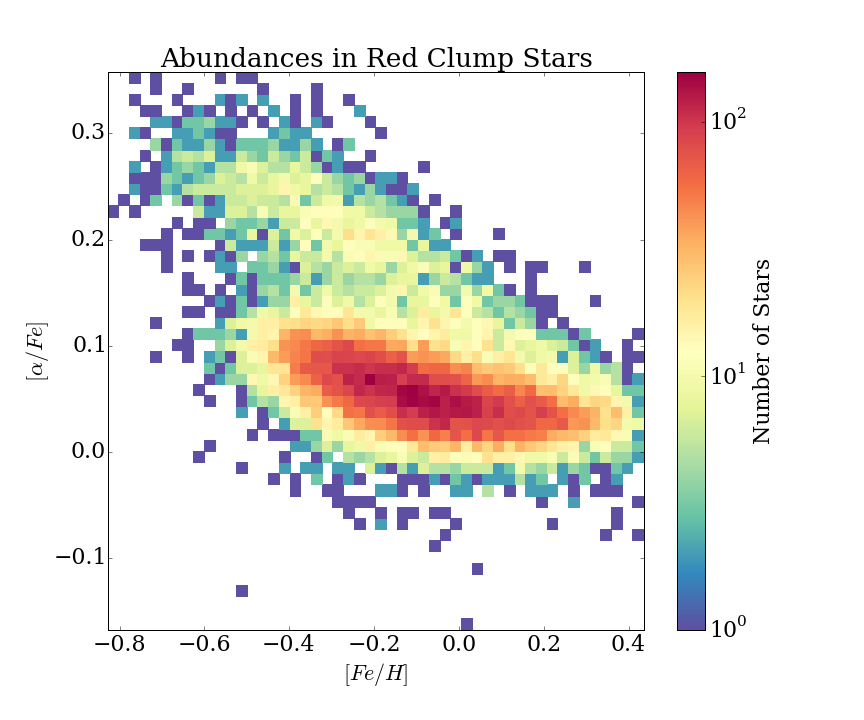
\includegraphics[width = 0.8\linewidth]{alpha_vs_fe.png}
\caption{$\alpha$-enhancement vs iron abundance for 19936 red clump stars from APOGEE Data Release 12.}
\end{centering}
\label{fig:abun}
\end{figure}

%\begin{figure}%[H]
%\begin{centering}
%\includegraphics[width = 0.8\linewidth]{samplerc.png}
%\caption{A sample spectrum from a red clump star. - ANY WAY TO MODIFY FONT SIZE EASILY}
%\end{centering}
%\label{fig:rc}
%\end{figure}


\bibliography{cite}

\end{document}